\documentclass[12pt,a4paper]{report}
\usepackage[pdftex]{graphicx}
\usepackage{url}
\usepackage{caption}
\usepackage{subcaption}
\usepackage{xargs}
\usepackage{amsmath,amssymb}
\usepackage{amsthm,amsfonts}
\usepackage{mathtools}
\usepackage{sectsty}
\usepackage{color}
\usepackage{diagbox}
\usepackage[
    bookmarks, 
    colorlinks=false, 
    pdfborder={0 0 0}, 
    pdftitle={Summer Internship Project}, 
    pdfauthor={Yannis Sauzeau}, 
    pdfsubject={Modeling the process of photosynthesis in leaf cells images}, 
    pdfkeywords={Internship Report Computer Science}
]{hyperref} 

\RequirePackage{doi}

\allsectionsfont{\raggedright}

\captionsetup[figure]{labelfont={small,bf},textfont=small}
\captionsetup[table]{labelfont={small,bf},textfont=small}

\counterwithout{figure}{chapter}
\counterwithout{table}{chapter}

\definecolor{green}{rgb}{0,0.5,0}
\def\green{\color{green}}
\definecolor{red}{rgb}{1,0,0}
\def\red{\color{red}}
\definecolor{blue}{rgb}{0,0,1}
\def\blue{\color{blue}}

\newcommandx{\diff} [2][1=x, 2=t]     {u({#1},{#2})}
\newcommandx{\coeff}[3][1=x, 2=t, 3=k]{c({#1},{#2},{#3})}
\newcommandx{\poly} [4][1=x, 2=t, 3=k, 4=0]{\sum_{{#3}={#4}}^{#2} \coeff[{#1}][{#2}][{#3}] \alpha^{#3}}

\newtheorem{definition}{Definition}

\begin{document}
\renewcommand\bibname{References} 


\begin{titlepage}

\begin{center}

\textup{\small {\bf Summer Internship Project} \\ Report}\\[0.3in]

% Title
\Large \textbf {Modeling the process of photosynthesis in leaf cells images}\\[0.7in]

% Submitted by
\normalsize Submitted by \\[0.2in]
\textbf{Yannis Sauzeau}\\
yannis.sauzeau@etu.univ-poitiers.fr\\
University of Poitiers\\

\vspace{.2in}
Under the guidance of\\[0.2in]
\textbf{Jiří Hladůvka}\\
jiri@prip.tuwien.ac.at\\
\vspace{0.1cm}
\textbf{Walter G. Kropatsch}\\
krw@prip.tuwien.ac.at\\
\vspace{0.1cm}
\textbf{Thierry Urruty}\\
thierry.urruty@univ-poitiers.fr



\vspace{.3in}

% Bottom of the page

\includegraphics[width=0.2\textwidth]{figures/prip.png}\\[0.1in]
\Large{
TU Wien\\
\vspace{0.1cm}
Faculty of Informatics\\
\vspace{0.1cm}
Institute of Visual Computing and Human-Centered Technology}\\
\normalsize
\vspace{0.25cm}
\textsc{Pattern Recognition and Image Processing Group}\\
\vspace{0.15cm}
Favoritenstr. 9/5. Stock/Stiege 2/E193-03\\
A-1040 Vienna, Austria \\

\end{center}

\end{titlepage}

\vspace{2in}
\begin{abstract}



\end{abstract} 


\pagenumbering{roman}
\tableofcontents


\newpage
\pagenumbering{arabic} 

\chapter{Objective}

This internship had several personal objectives:

\begin{itemize}
    \item Discover the world of research in the field of computer vision in
    a scientific way.
    \item Put into practice my knowledges acquired during my bachelor and my
    first year of master.
    \item Develop my english skills in order to be able to communicate with
    the world of research.
\end{itemize}
%
The technical objective of the internship was to contribute to an interdisciplinary
research project bridging plant biology, 3D imaging, and computer science. The 
objective of this project is to make a collaboration between the plant biologists
and the computer scientists in order to understand better the biological processes
involved in the photosynthesis of the plant. With this understanding, we will be able 
to reduce the amount of water we give to the plant for the growing process.
 
\chapter{Introduction}

\section{PRIP Laboratory}

\subsection{Presentation}

The Pattern Recognition and Image Processing Laboratory (PRIP) is a research
group of the Vienna University of Technology (TU Wien) and is part of the
Computer Science department. The TU Wien is Austria's largest research and 
educational institution in the field of technology and natural sciences.
The Computer Science department is one of Europe's leading research and innovation 
institutions. PRIP Laboratory is focused on advanced image representations and methods 
that allow the structure of the image to become an essential part of recognition systems.
Among the people working in the PRIP Laboratory are:

\begin{itemize}
    \item Prof. Walter G. Kropatsch, Head of the Group.
    \item Dr. Jiří Hladůvka, My tutor.
    \item Majid Banaeyan, PhD student.
    \item Darshan Batavia, PhD student.
\end{itemize}

\subsection{\textit{Water's gateway to heaven} project}

\textit{Water's gateway to heaven} is an interdisciplinary research project funded 
through the Life Sciences programme on Multimodal Imaging of the Vienna Science and 
Technology Fund (WWTF) \cite{WWTF}. The project is a collaboration between three Viennese 
universities: 

\begin{itemize}
    \item Plant ecophysiologists and anatomists at the University of Natural Resources 
    and Life Sciences \cite{BOKU}.
    \item Plant cell biologists at the University of Vienna \cite{UVI}.
    \item Computer scientists expert in pattern recognition and image analysis at the 
    Vienna University of Technology (TU Wien) \cite{TUV}.
\end{itemize}
%
The project focusses on the stomata, tiny pores on the surface of plant leaves. 
Stomata open and close to provide $\mathrm{CO_2}$ for photosynthesis and to limit 
water loss. This project uses novel temporal $3D$ imaging to provide a better description 
of stomatal movements in order to get a mechanistic understanding of how transient 
this movement. The goal is to answer long-standing questions about stomatal movements 
and to generate basic knowledge on how to improve stomatal responses under dynamic 
environments in order to increase net productivity and water-use efficiency \cite{WGH}.
         
\section{Technical overview}

The images use for this project are $3D$ images of leaves coming from high-resolution 
X-ray micro-tomography (micro-CT) and fluorescence microscopy. The size of the images is
$2000 \times 2000 \times 2000$ pixels. In order to track the change of the individual 
cells over time, hierarchies of abstract topological cell complexes are used, which will
reduce the image data to a neighboring structure of the plant cells without losing the
relation to the original data. This makes it possible to verify hypotheses at any time
that arise during the course of the biological analysis but may not have been known at
the time the hierarchy was built. Furthermore, this structure of the plant cells is to be
used to simulate dynamic processes \cite{PWGH}.

\subsection{Generalized maps}

The data structure chosen for this project is the $n$-dimensional generalized map
($n$-Gmap). An $n$-Gmap is a combinatorial data structure allowing to describe an
$n$-dimensional orientable or nonorientable quasi-manifold with or without boundary
\cite{Lienhardt}. This data structure is defined by a set of darts $D$ on which act
$n+1$ involutions $\alpha_i$ satisfying composition constraints of the following
definition \cite{Damiand}:

\begin{definition}[$n$-Gmap]
    An $n$-Gmap with $0<n$, is an $(n+2)$-tuple $G=(D,\alpha_0,\ldots,\alpha_{n})$ where:
    \begin{enumerate}
        \item $D$ is a finite set of darts;
        \item $\forall i\in\{0,\ldots,n\}:\alpha_i$ is an involution on $D$;
        \item $\forall i\in\{0,\ldots,n-2\},\forall j\in\{i+2,\ldots,n\}:
        \alpha_i \circ \alpha_j$ is an involution on $D$.
    \end{enumerate}
    \label{definition:gmap}
\end{definition}

\subsubsection{Python implementation}

For the project, PRIP has provided an implementation in Python based on the algorithms 
described in \cite{Lienhardt}. It consists in a hierarchy of classes which have their
root in the \textit{nGmap} class, that is an array based implementation of the
gmap, where a set of arrays is used to store the involutions. The \textit{PixelMap} class 
extends \textit{nGmap} and is a 2-Gmap representing an RxC image grid. The 
\textit{LabelMap} class extends \textit{PixelMap} and adds the possibility to build a 
2-Gmap representing an RxC image grid from a list of labels. This last class is very
useful for the project because it allows to convert the micro-CT images into a 2-Gmap
with the labels of the different leaf cells. After that we can easily make operations
on this 2-Gmap and apply image processing algorithms on it.

\subsection{Geodesic Distance Transform}

The Geodesic Distance Transform (GDT) computes distances within the connected
component of interest in a labeled image. The objects of interest are considered as
the foreground objects and the remaining objects are considered as background.
The computation of the GDT in a Gmap can be done in parallel with a logarithmic
time complexity \cite{Banaeyan}. We can compute the GDT on a labeled leaf image
to know the distance between the stomata and the mesophyll cells where the 
photosynthesis takes place. The stomata act as gates to control the amount of
$\mathrm{CO_2}$ that is released. The $\mathrm{CO_2}$ propagates through the
airspace to reach the mesophyll cells. On the \textbf{Figure \ref{fig:gdt}} we inialized
the seed label as the stomata connected component and we computed the GDT
on the airspace propagation label and mesophyll cells as the target label.

\begin{figure}[ht]
    \centering
    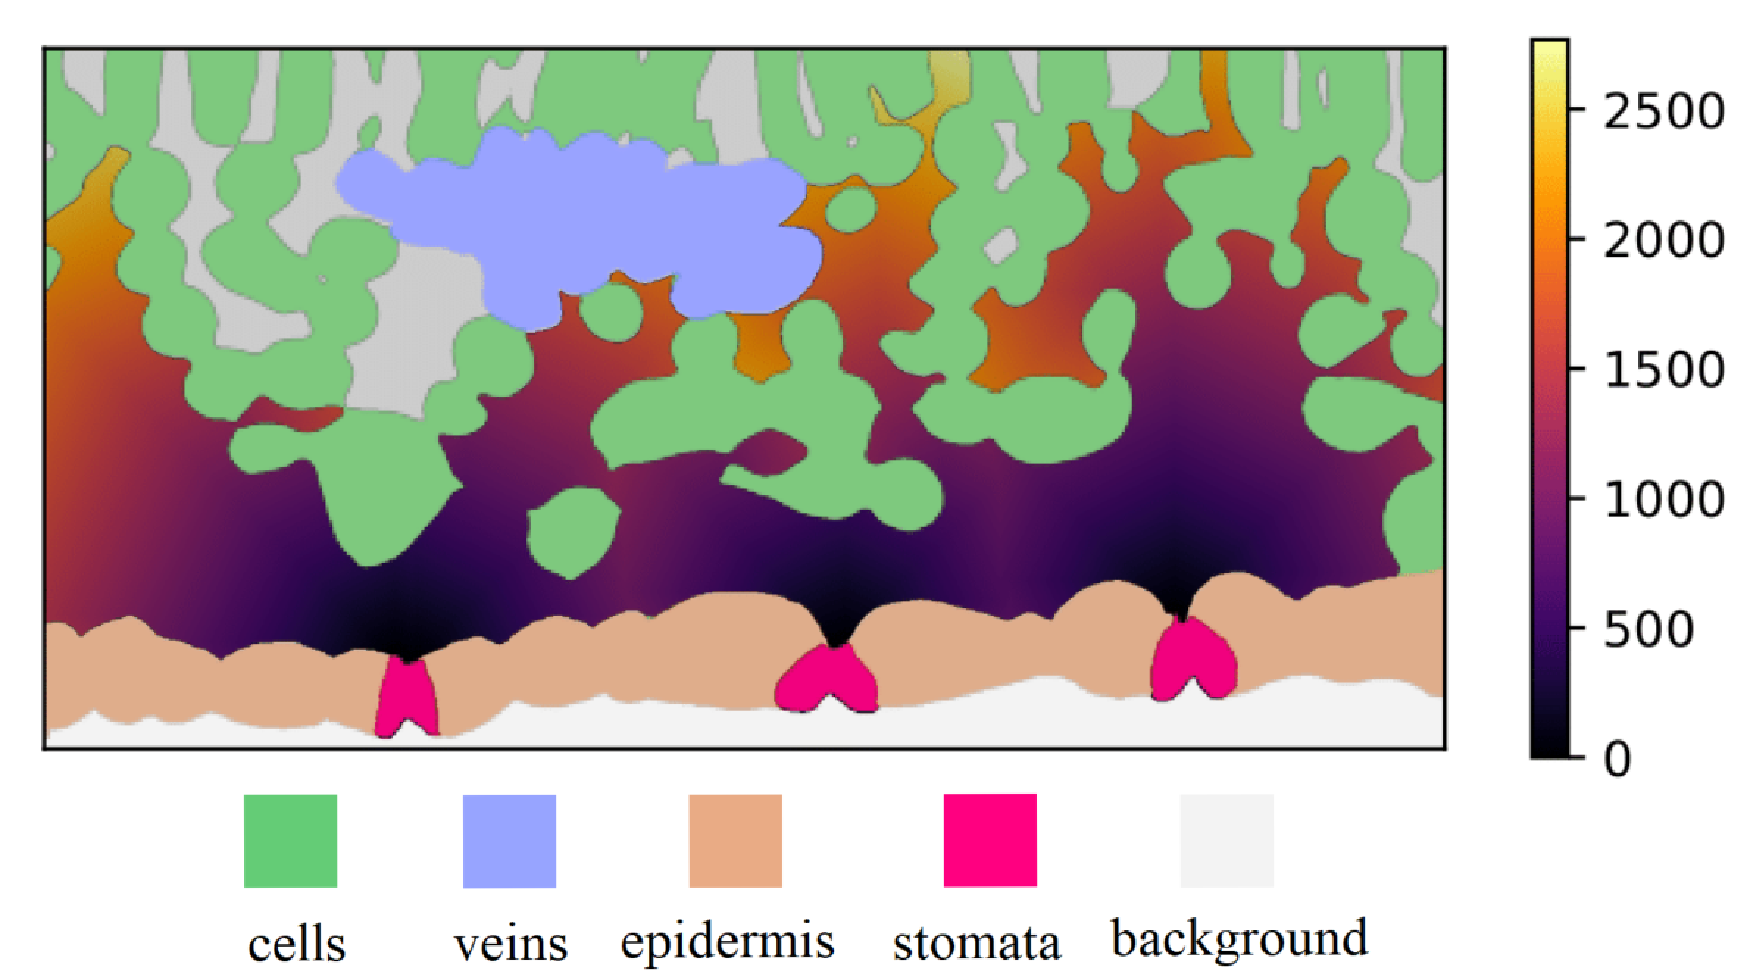
\includegraphics[width=0.8\textwidth]{figures/dt_color.pdf}
    \caption{GDT from stomata to mesophyll cells through the airspace}
    \label{fig:gdt}
\end{figure}

 
\chapter{Work Done}
 
\section{First work}

During the first month, my work was mainly focused on being familiar with the
project and the data, in order to find the best way to contribute to the project.

\subsection{Python library}

Carmine Carratù, the previous ERASMUS student, has been working on algorithms for the
computation of distance transform into $n$-Gmaps. My goal was to understand the code
and know how to use it to create figures for future publications. The code was not
documented so in reading the code I started to comment it and create documentation.
I also bring some optimizations to the code. Some functions was not very helpful for
the purpose of the project and the code was in several files, whereas we wanted to
keep the code as simple as possible in one notebook. So I created this notebook to
combine all the usefful and documented functions in one place.

\subsubsection{New representation on a $n$-Gmap}

\begin{figure}[ht]
    \centering
    \begin{subfigure}{0.49\textwidth}
        \centering
        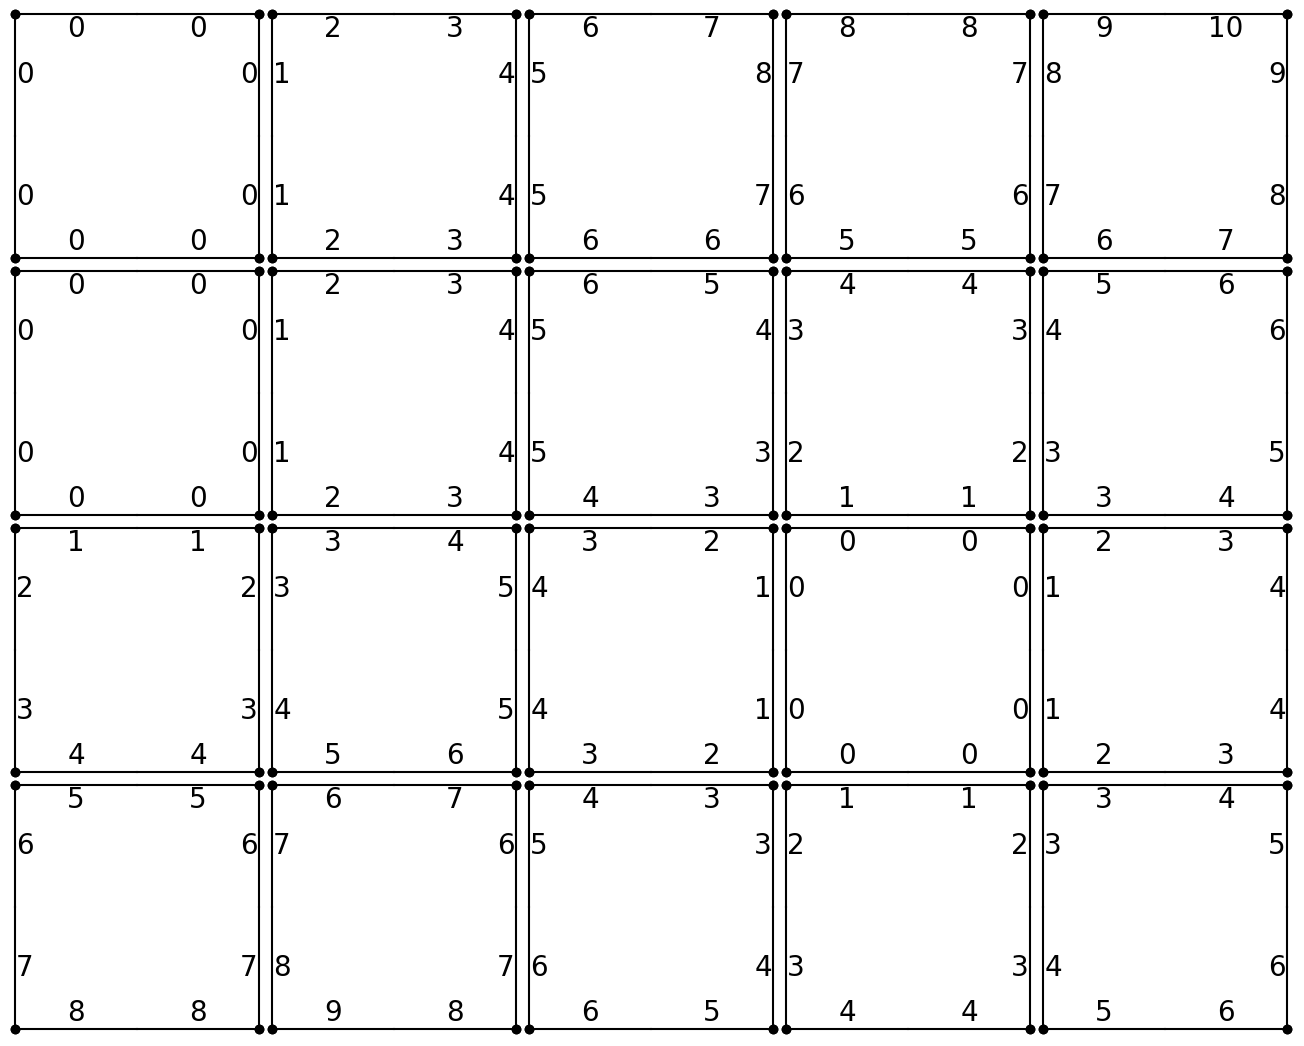
\includegraphics[width=\textwidth]{figures/gmap_dt_old.png}
        \caption{Old representation}
        \label{fig:gmap_dt_old}
    \end{subfigure}
    \hfill
    \begin{subfigure}{0.49\textwidth}
        \centering
        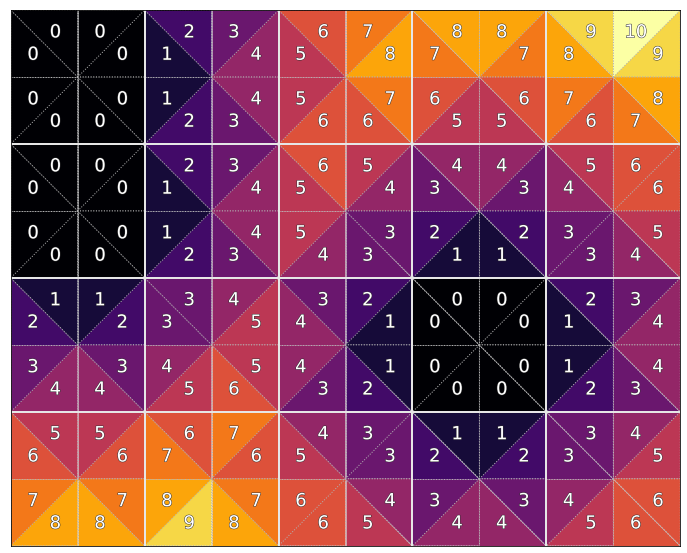
\includegraphics[width=\textwidth]{figures/gmap_dt_new.png}
        \caption{New representation}
        \label{fig:gmap_dt_new}
    \end{subfigure}
    \caption{Different representations of the distance transform on a $n$-Gmap}
    \label{fig:gmap_dt}
\end{figure}

The representation of the distance transform was changed to be more intuitive. On
the figure (\ref{fig:gmap_dt_old}) the distance transform is represented as a
$n$-Gmap with the distance values on the dart. It's hard to see the variation of the
distance values. The new representation is shown in the figure (\ref{fig:gmap_dt_new}).
This representation uses triangles for each dart showing the distance values. In
addition, we use the \textit{inferno} color map that is perceptually uniform with 
monotonically increasing luminance \cite{Moreland}.

\subsubsection{New representation on a leaf image}

\begin{figure}[ht]
    \centering
    \begin{subfigure}{0.45\textwidth}
        \centering
        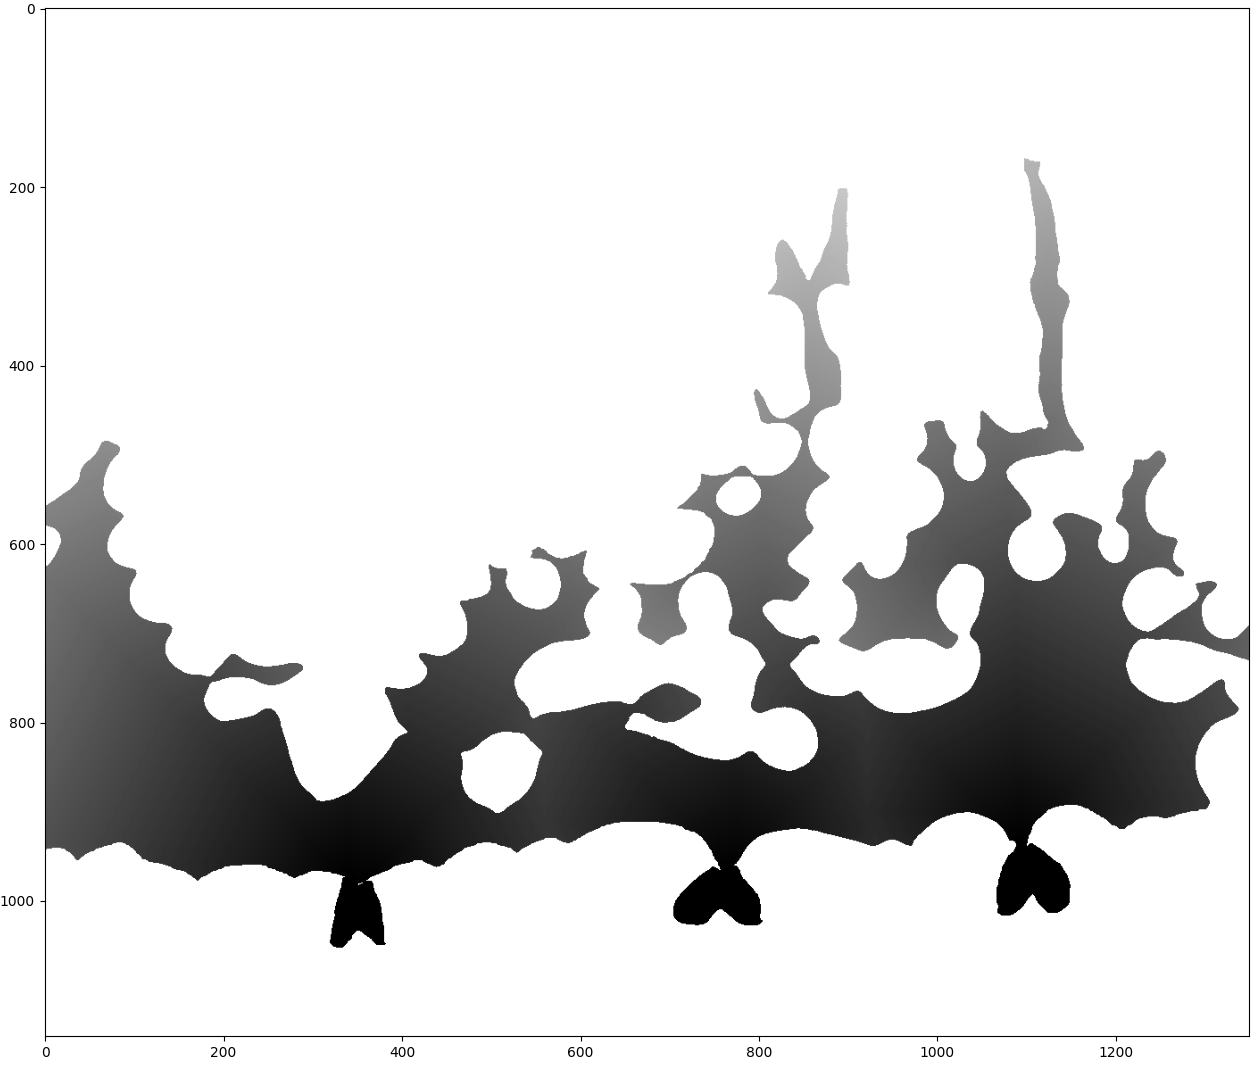
\includegraphics[width=\textwidth]{figures/leaf_dt_old.png}
        \caption{Old representation}
        \label{fig:leaf_dt_old}
    \end{subfigure}
    \hfill
    \begin{subfigure}{0.54\textwidth}
        \centering
        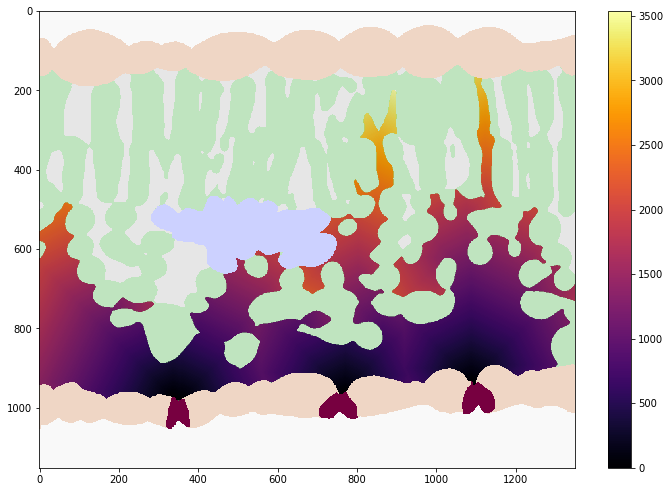
\includegraphics[width=\textwidth]{figures/leaf_dt_new.png}
        \caption{New representation}
        \label{fig:leaf_dt_new}
    \end{subfigure}
    \caption{Different representations of the distance transform on a leaf}
    \label{fig:leaf_dt}
\end{figure}

On the leaf image, the representation was changed too. Before the distance transform
was print with a black and grey color map as shown in the figure (\ref{fig:leaf_dt_old}). 
The new representation, shown in the figure (\ref{fig:leaf_dt_new}) uses the 
\textit{inferno} color map and an overlay can be seen to show the other parts of the 
leaf image.

\subsubsection{Wave propagation animation}

\begin{figure}[ht]
    \centering
    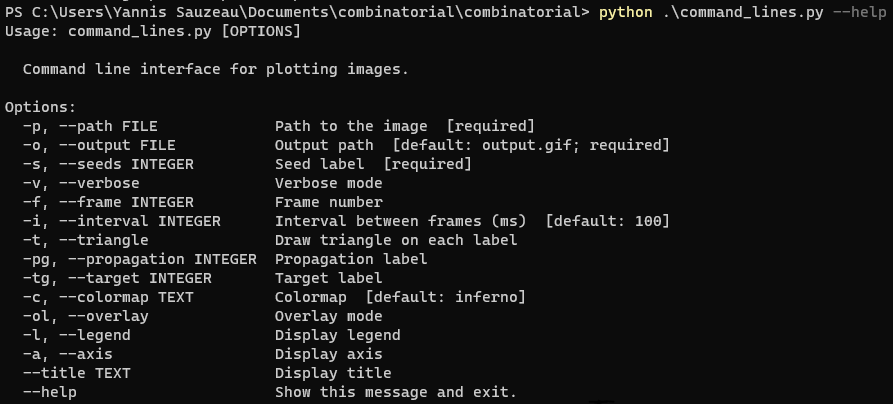
\includegraphics[width=\textwidth]{figures/cli.png}
    \caption{Command line program for wave propagation animation}
    \label{fig:cli}
\end{figure}

The distance transform algorithm uses a wave propagation method to propagate the
distance values. I used \textit{Click} \cite{CLICK} Python package to create a
command line program that can be used to animate the propagation of the distance
transform. On the figure (\ref{fig:cli}) the different options for the command line
program are shown. Among this options, we have the required integer for the seed
label, it's form the pixel with this label that the wave will start propagating.
The propagation label integer corresponds to the pixel with this label that the wave
will propagate to, and the target label integer is the same but for the target pixel.

\subsection{Diffusion equation}

In order to achieve the main goal of the Watergate project it's important to study the
gas exchange process that occurs in plant leaves. The distance transform is used to
compute the geodesic distance from stomata to mesophyll cells where the photosynthesis
is performed. The gas exchange rate depends on this distance over which the diffusion 
occurs \cite{RSB}. To study gas exchanges inside leaves, we have chosen the diffusion
equation, described in 2D by this Partial Differential Equation (PDE):
%
\begin{equation}
  \frac{\partial u}{\partial t} = \alpha \left( \frac{\partial^2u}{\partial x^2} + \frac{\partial^2u}{\partial y^2} \right)
  \label{eq:heat}
\end{equation}
%
where $u(x,y,t)$ is the concentration at position $x$, $y$ in time $t$ and $\alpha$ is the
diffusion coefficient.

\subsubsection{Iterative solution}

With a finite-difference method, we can convert the PDE \eqref{eq:heat} into an explicit 
equation described as follows:
%
\begin{multline}
    u(x,y,t+1) = u(x,y,t) + \alpha \big(
        u(x+1,y,t) + u(x-1,y,t) \\
        + u(x,y+1,t) + u(x,y-1,t) 
        - 4 u(x,y,t)
        \big)
    \label{eq:iterative}
\end{multline}
%
where $\Gamma(x)$ is the set of neighbors of pixel $x$.

\section{Modeling the Diffusion of \texorpdfstring{$\mathrm{CO_2}$}{CO2} inside Leaves}

\subsection{1D Diffusion}

The diffusion equation in 1D becomes
%
\begin{equation}
    \diff[x][t+1] = \diff + \alpha \big(\diff[x-1] + \diff[x+1] - 2 \diff \big)
    \label{eq:1D:iterative}
\end{equation}
%
where $t \ge 0$ is the iteration count and $x$ the pixel index along the sequence. 
%
We assume that the total gas volumes \eqref{eq:associativity} of both sequences 
does not change by the diffusion, e.g. for all iterations $t$.
%
\begin{equation}\label{eq:associativity}
    \sum_x \diff = \sum_x \diff[x][0]
\end{equation}
%
Diffusion propagates in both directions (increase and decrease of index) symmetrically.
Consequently we have for all iterations before reaching the end of the sequence:
%
\begin{equation}\label{eq:symmetry}
    \diff[x] + \diff[y] = L+H \quad \mbox{ for all } x+y=1
\end{equation}

\subsubsection{Sequence initialization}

Consider one 1D sequence of 2-connected pixels without self-intersection.
Let's note $x$ the index along the sequence and $\diff$ the concentration at the 
time $t$. The first half ($x \le 0$) should be filled with a high concentration
of $\mathrm{CO_2}$, $H$, and the second half ($x > 0$) with low concentration 
of $\mathrm{CO_2}$, $L$:

\begin{table}[ht]
    \centering
    \begin{tabular}{|c|c|c|c|c|c||c|c|c|c|c|} \hline
        $x$           & $\ldots$ &-3 &-2 &-1 & 0 & 1 & 2 & 3 & 4 & $\ldots$ \\ \hline \hline
        $\diff[x][0]$ & $\ldots$ & H & H & H & H & L & L & L & L & $\ldots$ \\ \hline
    \end{tabular}
    \caption{Sequence initialization}
    \label{tab:init}
\end{table}

\subsubsection{Normalized formula}

Setting $\alpha=1$ we notice that $\diff$ starts oscillating 
around the boundary between $L$ and $H$ already at the second iteration:

\begin{table}[ht]
    \centering
    $$
        \begin{array}{|l|c|c|c|c|c||c|c|c|c|c|} \hline
        x&\ldots &-3 &-2 &-1   & 0   & 1    & 2   & 3 & 4 & \ldots \\ \hline \hline
        0&\ldots & H & H & H   & H   & L    & L   & L & L & \ldots \\ \hline
        1&\ldots & H & H & H   & L   & H    & L   & L & L & \ldots \\ \hline
        2&\ldots & H & H & L   &2H-L & 2L-H & H   & L & L & \ldots \\ \hline
        3&\ldots & H & L &3H-2L&4L-3H& 4H-3L&3L-2H& H & L & \ldots \\ \hline 
        \end{array}
    $$
    \caption{Result with $\alpha=1$}
    \label{tab:1D:result_a1}
\end{table}

The calculated values, $2H-L>H$, $2L-H<L$, are outside the interval $[L,H]$.
The reason is that the differences to the center pixels need to be normalized, or
equivalently the range of $\alpha \in [0,1/2]$ in 1D. The same result with $\alpha=1/2$:

\begin{table}[ht]
    \centering
    $$
        \begin{array}{|l|c|c|c|c|c||c|c|c|c|c|} \hline
        x&\ldots&       -3       &       -2       &       -1        &       0         &       1         &       2         &       3        &       4        &\ldots\\\hline \hline
        0&\ldots&        H       &        H       &        H        &       H         &       L         &       L         &       L        &       L        &\ldots\\\hline
        1&\ldots&        H       &        H       &        H        & \frac{H+L}{2}   & \frac{L+H}{2}   &       L         &       L        &       L        &\ldots\\\hline
        2&\ldots&        H       &        H       &  \frac{3H+L}{4} & \frac{3H+L}{4}  & \frac{3L+H}{4}  & \frac{3L+H}{4}  &       L        &       L        &\ldots\\\hline
        3&\ldots&        H       & \frac{7H+L}{8} &  \frac{7H+L}{8} & \frac{H+L}{2}   & \frac{L+H}{2}   & \frac{7L+H}{8}  & \frac{7L+H}{8} &       L        &\ldots\\\hline
        \end{array}
    $$
    \caption{Result with $\alpha=1/2$}
    \label{tab:1D:result_a0d5}
\end{table}

Notice that for $\alpha \le 1/2$ the monotonicity of the complete sequence is preserved.
The diffused values are linear combinations of $L$ and $H$ and remain within $[L,H]$.
The diffusion could be formulated with the neighborhood $\Gamma(x)$ for all indices $x$ 
as follows:
%
\begin{equation}\label{eq:1D:normalized}
    \diff[x][t+1] = \diff + \frac{\alpha}{|\Gamma(x)|} \sum_{n \in \Gamma(x)} \left(\diff[n] - \diff[x]\right)
\end{equation}
%
With this formula, $\alpha$ needs to be normalized to the range $[0,1]$. This formulation 
would also extend to higher dimensions.

\subsubsection{Wavefront formula}

We can derive direct formula (polynomials of degree $t$ and parameters $\alpha, x,$
$L, H$) for any iteration $t$ without the need to do the intermediate 
iterations within the first wave propagation, i.e. until the front reaches the end 
of the sequence. A simple formula for the front of the wave is:
%
\begin{equation}
    \diff[t][t] = (1 - \alpha^t)L + \alpha^t H
    \label{eq:wavefront}
\end{equation}
%
If $t$ is the result of the distance transform, then the value of the wavefront can be
computed directly without reference to intermediate results of previous iterations.

\subsubsection{Polynomial Basis Function}

More concretely, the weights of L and H for $t=0\ldots2,x=-2\ldots3$ can be expressed 
as polynomials of $\alpha$:

\begin{table}[ht]
    \small
    \centering
    $$
        \begin{array}{|c||c|c|c|} \hline
         x & \multicolumn{3}{|c|}{u(x,t)} \\ \hline \hline
         3 & L &          L           &                     L                       \\ \hline
         2 & L &          L           &         (1-\alpha^2)L+\alpha^2H             \\ \hline
         1 & L & (1-\alpha)L+\alpha H & (1-2\alpha+3\alpha^2)L+(2\alpha-3\alpha^2)H \\ \hline \hline
         0 & H & (1-\alpha)H+\alpha L & (1-2\alpha+3\alpha^2)H+(2\alpha-3\alpha^2)L \\ \hline
        -1 & H &          H           &         (1-\alpha^2)H+\alpha^2L             \\ \hline
        -2 & H &          H           &                     H                       \\ \hline \hline
        t  & 0 &          1           &                     2                       \\ \hline
        \end{array}
    $$
    \caption{Weights of $L$ and $H$ expressed with polynomials}
    \label{tab:weight_poly}
\end{table}

We observe that the coefficients $L$ and $H$ are symmetric with respect to $x=0.5$ and 
the polynomial of $L$ is $1-$ the polynomial of of $H$ for $x>0$. For $x\le0$, it's the 
opposite, i.e. the polynomial of $H$ is $1-$ the pronominal of $L$:
%
\begin{equation}
    \begin{split}
        \diff & = \poly L + (1 - \poly) H \\
              & = H - \left(\poly \right) (H-L)
    \end{split}
    \label{eq:polynomial}
\end{equation}
%
where $\coeff$ is the coefficient of the polynomial of degree $k$ at iteration $t$ and
$x$ is the index along the sequence.

\def\R{\red{0}} % blank zero
\def\G{\green{0}} % blank zero
\def\B{\blue{1}} % blank zero

\begin{table}[ht]
    \centering
    \begin{tabular}{|r||r|rr|rrr|rrrr|rrrrr|}
        \hline
        t & 0 & \multicolumn{2}{|c|}{1} & \multicolumn{3}{|c|}{2} &\multicolumn{4}{|c|}{3} &\multicolumn{5}{|c|}{4} \\ 
        \hline \hline
        \diagbox{x}{k}  & 0 & 0 & 1 & 0 & 1 & 2 & 0 & 1 & 2 & 3 & 0 & 1 & 2 & 3 & 4 \\
        \hline
        \hline
        4 & \B & \B & \G & \B & \G & \G & \B & \G & \G & \G & \B & \G & \G & \G & -1  \\
        3 & \B & \B & \G & \B & \G & \G & \B & \G & \G & -1 & \B & \G & \G & -4 &  7  \\
        2 & \B & \B & \G & \B & \G & -1 & \B & \G & -3 &  5 & \B & \G & -6 & 20 &-21  \\
        1 & \B & \B & -1 & \B & -2 &  3 & \B & -3 &  9 &-10 & \B & -4 & 18 &-40 & 35  \\
        \hline \hline
        0 & \R & \R &  1 & \R &  2 & -3 & \R &  3 & -9 & 10 & \R &  4 &-18 & 40  &-35 \\
        -1 & \R & \R & \R & \R & \R &  1 & \R & \R &  3 & -5 & \R & \R &  6 &-20 & 21 \\
        -2 & \R & \R & \R & \R & \R & \R & \R & \R & \R &  1 & \R & \R & \R &  4 & -7 \\
        -3 & \R & \R & \R & \R & \R & \R & \R & \R & \R & \R & \R & \R & \R & \R &  1 \\
        \hline
    \end{tabular}
    \caption{Coefficients $\coeff$ for the very first time steps ($t = 0 \ldots 4$).}
    \label{tab:coefficients}
\end{table}

Deriving the coefficients of the polynomial (Table \ref{tab:coefficients} shows the 
coefficients for the first 4 time steps), we arrived at the following closed-form 
involving binomial coefficients for negative arguments\footnote{Explaining the colored 
entries in Table \ref{tab:coefficients}} \cite{Kronenburg}.
%
\begin{equation}
  \coeff = (-1)^{1+x+k} \binom{t}{k} \binom{2k-1}{x+k-1}
  \label{eq:coefficients}
\end{equation}
%
With respect of property \eqref{eq:symmetry}, we have this property:
%
\begin{equation}
    \poly[x][t][k][1] = -\poly[y][t][k][1] \quad \mbox{ for all } x+y=1
    \label{poly_eq}
\end{equation}
%
With the property above, to know all the values of $\diff$ of a certain iteration $t$,
we only have to compute $\poly$ with $x\in[1,t]$.

\subsubsection{Result}

To study the diffusion of $\mathrm{CO_2}$ in the leaf from stomata to the leaf cells,
we first compute the distance transform $d(x)$ of each pixel $x \in R$ in the airspace $R$.
Afterward, we compute the coefficients $c(t,k,x)$ with $t = \max_{x \in R}d(x)$.
Once we have the coefficients, we can compute the concentration $u(x,t)$ by
\eqref{eq:coefficients}. The result is identical to the iterative solution and is visualized
in figure (\ref{fig:diffusion}).

\begin{figure}[ht]
    \centering
    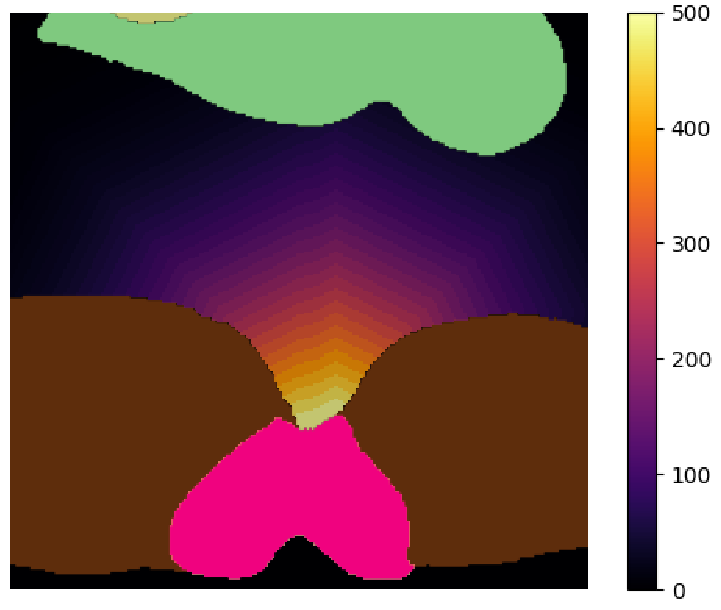
\includegraphics[width=0.75\linewidth]{figures/diffusion.pdf}
    \caption{Equation \eqref{eq:polynomial} used to describe the diffusion of $\mathrm{CO_2}$ from 
    stoma.}
    \label{fig:diffusion}
\end{figure}

Another point of interest is to compute only the diffusion values for the pixels corresponding to
the leaf cells border. Indeed, to know the concentration of the leaf cells, we don't need to 
compute the diffusion values for the other parts of the leaf.

\subsection{Stomata's movement}
\label{sec:stomata}

\begin{figure}[ht]
    \centering
    \begin{subfigure}[b]{0.49\textwidth}
        \centering
        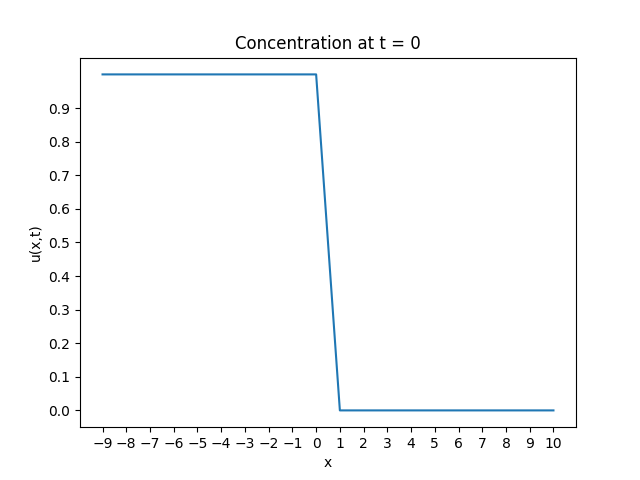
\includegraphics[width=\textwidth]{figures/concentration_at_t_0_size_20.png}
        \caption{$u(x,0)$}
        \label{fig:u_0}
    \end{subfigure}
    \hfill
    \begin{subfigure}[b]{0.49\textwidth}
        \centering
        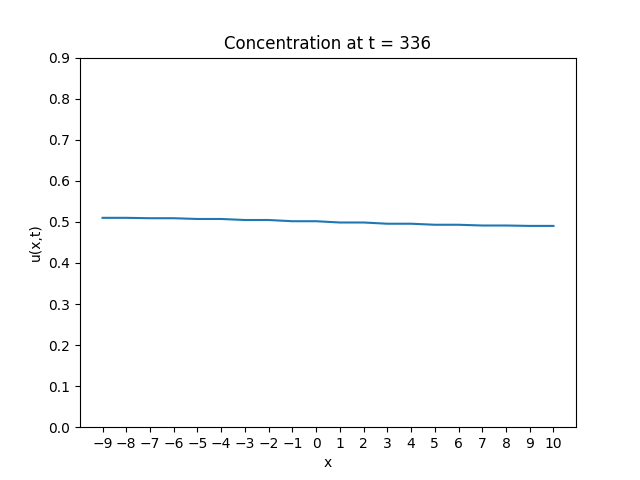
\includegraphics[width=\textwidth]{figures/concentration_at_t_336_size_20.png}
        \caption{$u(x,336)$}
        \label{fig:u_336}
    \end{subfigure}
    \caption{Concentration $u(x,t)$ in a sequence of size 20 at the initialization and near
    the stabilized state}
    \label{fig:seq_20}
\end{figure}

In this section we will study the effects of the movement of the stomata. Let's start 
with a simple example. First, initialize a sequence like in Table \ref{tab:init}. The size 
of the sequence is 20 pixels with $x \in [-9,10]$, $H=100\%$, $L=0\%$ and $t=0$ (see the 
figure (\ref{fig:u_0})). This sequence represents a closed stoma at the position $x=0$, 
the pixels with negative index are the ones outside the leaf and the ones with positive 
index are the ones inside the leaf. When $t>0$ the stoma is open. Using the iterative 
method (\ref{eq:1D:normalized}) with $\alpha = 1$ we want to know the time $t$ when the 
end of the sequence is near to be stabilized, i.e. that the value at the end of the 
sequence is greater than $49\%$. This value is reached at time $t=336$ (see the figure 
(\ref{fig:u_336})).

\subsubsection{Different sequence sizes}

We want to know if the size of the sequence influences the time taken to reach the
stabilized state. We use the same method as above but with different sizes of sequence.
For 10 pixels, the stabilized state is reached at time $t=83$, for 50 pixels at time 
$t=2103$ and for 100 pixels at time $t=8416$. With a size of 10 pixels the time taken to 
reach the stabilized state is much smaller than with a size of 50 pixels and with a size 
of 100 pixels. With the sequence of 100 pixels it takes 100 times longer to reach the 
stabilized state than with the sequence of 10 pixels.

\subsubsection{Function to calculate the time taken to reach the stabilized state}

The table below shows the time taken to reach the stabilized state for the first 
sequences from 2 to 10 pixels. The figure (\ref{fig:s_time}) shows this function
for sequences between 2 and 100 pixels.

\begin{table}[ht]
    \centering
    \begin{tabular}{|l|c|c|c|c|c|c|c|c|c|} \hline
        number of pixels in the sequence   & 2 & 3 & 4 & 5 & 6 & 7 & 8 & 9 & 10 \\\hline
        time to reach the stabilized state & 1 & 6 & 12 & 20 & 29 & 40 & 52 & 67 & 83 \\\hline
    \end{tabular}
    \caption{Time to reach the stabilized state for first 8 sequences of sizes between 2 and 10 pixels}
    \label{tab:s_time}
\end{table}

Let's see if sequence of time obtained from the table can be computed from the number of 
pixels. To know if the time to reach the stabilized state can be computed from the number 
of pixels we can see if it's a polynomial function. To that we can compute the difference 
table (\ref{tab:diff_s_time}). We can observe that the differences didn't converge to a 
constant value. This is because the time to reach the stabilized state is not a polynomial 
function.

\begin{table}[ht]
    \centering
    \begin{tabular}{ccccccccccc}
        1 &   & 6 &   & 12 &    & 20       &          & 29       &         & \red{36}\\
          & 5 &   & 6 &    & 8  &          & 9        &          & \red{7} &\\
          &   & 1 &   & 2  &    & 1        &          & \red{-2} &         &\\
          &   &   & 1 &    & -1 &          & \red{-3} &          &         &\\
          &   &   &   & -2 &    & \red{-2} &          &          &         &\\
    \end{tabular}
    \caption{Difference table for the time to reach the stabilized state for the first 5 sequences of sizes between 2 and 6 pixels}
    \label{tab:diff_s_time}
\end{table}

\begin{figure}[ht]
    \center
    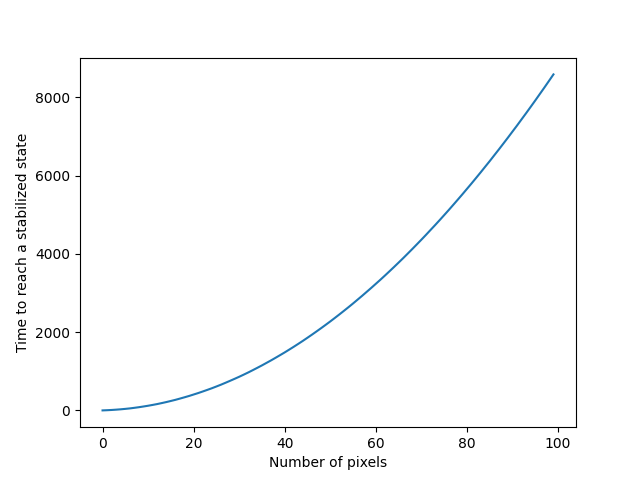
\includegraphics[width=0.66\textwidth]{figures/function_to_reach_a_stabilized_state.png}
    \caption{Function to reach a stabilized state from different sizes of sequence}
    \label{fig:s_time}
\end{figure}

\subsubsection{Stomata closing after few iterations}

\begin{figure}[htb]
    \center
    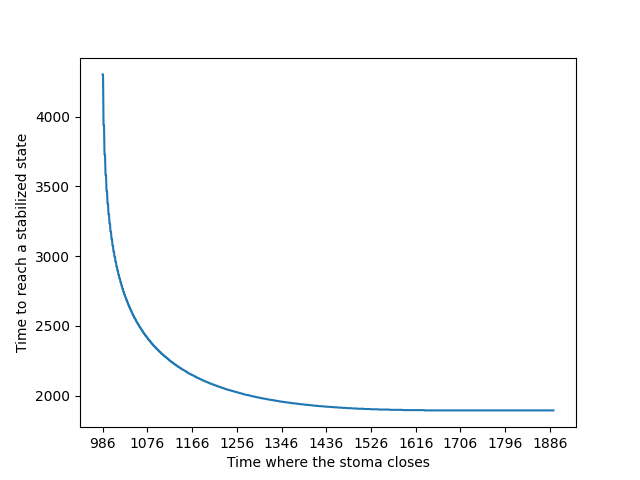
\includegraphics[width=0.66\textwidth]{figures/function_to_reach_a_stabilized_state_when_the_stoma_closes.png}
    \caption{Function to reach a stabilized state when the stoma closes after $x$ iterations}
    \label{fig:s_time_close}
\end{figure}

We want to know if the stabilized state is reached faster when the stomata close after
few iterations. We start with a sequence of 100 pixels and we want to know the number
of iterations needed to the end of the sequence reach the value of 25\% when the stoma
is always open end when the stoma close after few iterations. When the stoma is open
we need time $t=1894$ to reach the value of 25\%. On the figure 
(\ref{fig:s_time_close}), we can see that for reaching the value of 25\% the stoma
need to be close after time $t=986$. When the stoma closes at time $t=1000$, we need 
$t=4000$ to reach the value of 25\%, i.e. more than two times the time needed to reach
the same value when the stoma is open. More the stoma takes time to close, less we 
need time to reach the value of 25\%. When we close the stoma at time after $t=1650$,
then the time to reach the value of 25\% is constant and equal to $t=1894$.

\subsection{Simulate the diffusion problem for higher dimensions}

Let's transform our 1D sequence into a 2D sequence. We can do this by creating a
matrix with the same size as the 1D sequence and filling it with the values of the 
1D sequence. Let's note $x$ the index of the pixel in the 1D sequence and $y$ the index 
of the pixel in the 2D sequence, and $u(x,y,t)$ the concentration at the iteration $t$.
To differentiate the notation between the diffusion in the 1D and 2D case, we will use
$u_{1D}(x,t)$ for the 1D diffusion and $u_{2D}(x,y,t)$ for the 2D diffusion.
We will initialize the matrix with $u_{2D}(x,y,0) = u_{1D}(x,0)$ like the table below:

\begin{table}[htb]
    \centering
    \begin{tabular}{|c|c|c|c|c|c||c|c|c|c|c|} \hline
        $u(x,0,0)$&\ldots&   H  &   H  &   H  &   H  &   L  &   L  &   L  &   L  &\ldots\\\hline
        $u(x,1,0)$&\ldots&   H  &   H  &   H  &   H  &   L  &   L  &   L  &   L  &\ldots\\\hline 
        $u(x,2,0)$&\ldots&   H  &   H  &   H  &   H  &   L  &   L  &   L  &   L  &\ldots\\\hline 
        \ldots    &\ldots&\ldots&\ldots&\ldots&\ldots&\ldots&\ldots&\ldots&\ldots&\ldots\\\hline 
        $u(x,y,0)$&\ldots&   H  &   H  &   H  &   H  &   L  &   L  &   L  &   L  & \ldots \\ \hline \hline
        $x$       &\ldots&  -3  &  -2  &  -1  &   0  &   1  &   2  &   3  &   4  & \ldots \\ \hline
    \end{tabular}
    \caption{2D sequence initialization}
    \label{tab:2D_init}
\end{table}

\subsubsection{2D formula idealistic model}

Let's adapt the formula (\ref{eq:1D:normalized}) to the 2D diffusion problem:

\begin{equation}
    u_{2D}(x,y,t+1) = u_{2D}(x,y,t) + \frac{\alpha}{|\Gamma(x,y)|} \sum_{n,m \in \Gamma(x,y)} \left(u_{2D}(n,m,t) - u_{2D}(x,y,t)\right)
    \label{eq:2Dnorm}
\end{equation}
%
With $\Gamma(x,y)$ the set of all the pixels that are connected to the pixel $(x,y)$. \\
%
Now we can compute the diffusion for the 2D sequence and compare the results with the 
1D sequence. For the computation we will take $\alpha = 1$ and $t = 100$. The results
(figure (\ref{fig:diff_1d_vs_2d_100})) show that with the same alpha, the diffusion
is two time faster in the 1D sequence than in the 2D sequence. It's understandable since
the 1D diffusion only propagate in two directions and the 2D diffusion propagate in four
directions. When we compare the results of the first iterations in the 1D and 2D sequences
with the table (\ref{tab:1D:result_a0d5}) in 1D and table (\ref{tab:result_2d_1a}) in 2D,
we can see similarity. For instance, $u_{2D}(1,y,1)=u_{1D}(2,2)$, $u_{2D}(1,y,2)=u_{1D}(2,4)$,
or $u_{2D}(2,y,2)=u_{1D}(4,4)$. We can generalize by the formula:

\begin{equation}
    u_{2D}(x,y,t)=u_{1D}(2x,2t) 
    \label{eq:2D_1D_basic}
\end{equation}
%
The formula below is working only with specific conditions, i.e. $u_{2D}(x,y,0)=u_{1D}(x,0)$
and $u_{2D}(x,y-1,t)=u_{2D}(x,y,t)=u_{2D}(x,y+1,t)$.

\begin{figure}[ht]
    \centering
    \begin{subfigure}[b]{0.49\textwidth}
        \centering
        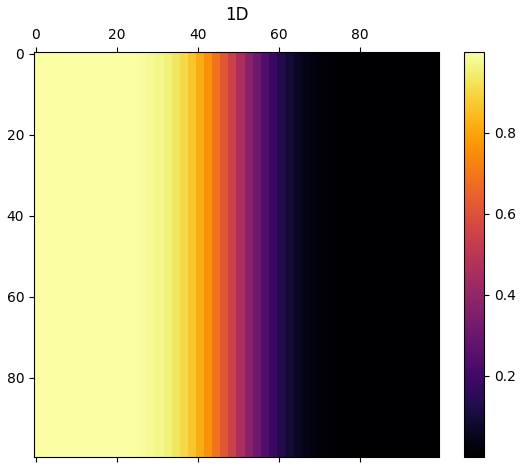
\includegraphics[width=\textwidth]{figures/1d_100t_1a.png}
        \caption{Diffusion with $\alpha = 1$ in 1D sequence of size $100$}
        \label{fig:diff_1d_100}
    \end{subfigure}
    \hfill
    \begin{subfigure}[b]{0.49\textwidth}
        \centering
        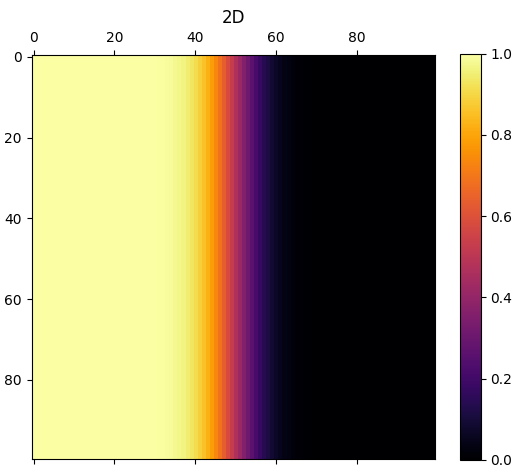
\includegraphics[width=\textwidth]{figures/2d_100t_1a.png}
        \caption{Diffusion with $\alpha = 1$ in 2D sequence of size $100 \times 100$}
        \label{fig:diff_2d_100}
    \end{subfigure}
    \caption{Diffusion with $\alpha = 1$ in 1D and 2D sequence of size $100 \times 100$}
    \label{fig:diff_1d_vs_2d_100}
\end{figure}

\begin{table}[ht]
    \centering
    $$
        \begin{array}{|l|c|c|c|c||c|c|c|c|} \hline
        x       &\ldots&-2&       -1       &        0        &        1        &        2       &3&\ldots\\\hline \hline
        u(x,y,0)&\ldots& H&        H       &        H        &        L        &        L       &L&\ldots\\\hline
        u(x,y,1)&\ldots& H&        H       & \frac{3H+L}{4}  & \frac{3L+H}{4}  &        L       &L&\ldots\\\hline
        u(x,y,2)&\ldots& H&\frac{15H+L}{16}&\frac{11H+5L}{16}&\frac{11L+5H}{16}&\frac{15L+H}{16}&L&\ldots\\\hline
        \end{array}
    $$
    \caption{Result with $\alpha=1$ in 2D sequence}
    \label{tab:result_2d_1a}
\end{table}

\subsubsection{General 2D formula}

\begin{figure}[ht]
    \centering
    \begin{subfigure}[b]{0.49\textwidth}
        \centering
        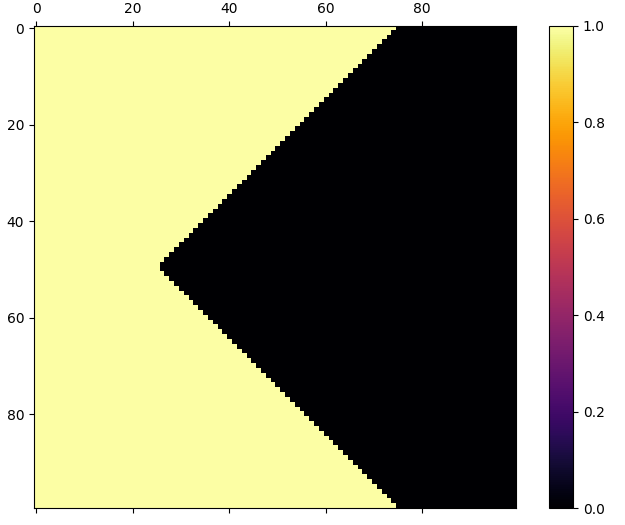
\includegraphics[width=\textwidth]{figures/2d_pyramid_init.png}
        \caption{2D funnel sequence at the initialization}
        \label{fig:diff_2d_fnl_init}
    \end{subfigure}
    \hfill
    \begin{subfigure}[b]{0.47\textwidth}
        \centering
        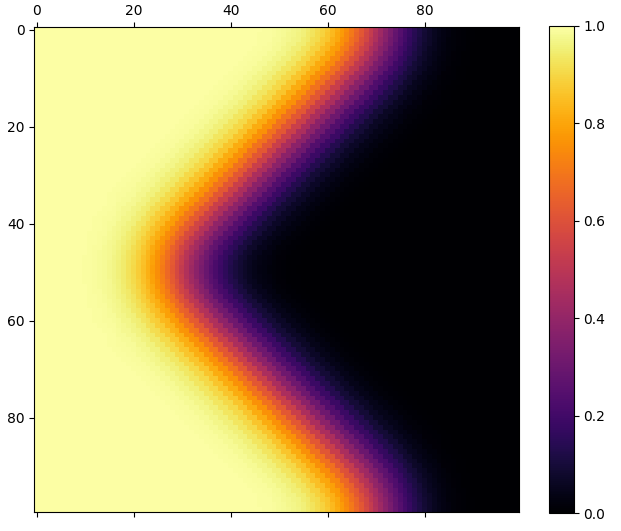
\includegraphics[width=\textwidth]{figures/2d_pyramid_100.png}
        \caption{Diffusion with $\alpha=1$ in 2D funnel sequence at iteration $100$}
        \label{fig:diff_2d_fnl_100}
    \end{subfigure}
    \caption{Diffusion in 2D sequence of size $100 \times 100$ more near the stomata shape}
    \label{fig:diff_fnl_pyr}
\end{figure}

The shape of stomata is like a funnel, so let's create a 2D sequence of size $100 
\times 100$ that looks like a funnel. The figure (\ref{fig:diff_2d_fnl_init}) shows the 
initial sequence. Here the formula \eqref{eq:2D_1D_basic} is not working, but we can find
a formula that works for every pixel. Let's start some observations. On the first step 
for the 1D diffusion we can isolate two different configurations that makes changes in 
the sequence. Each of this configuration leads to four variations in the 2D sequence:

\begin{figure}[ht]
    \centering
    \begin{subfigure}[b]{1\textwidth}
        \centering
        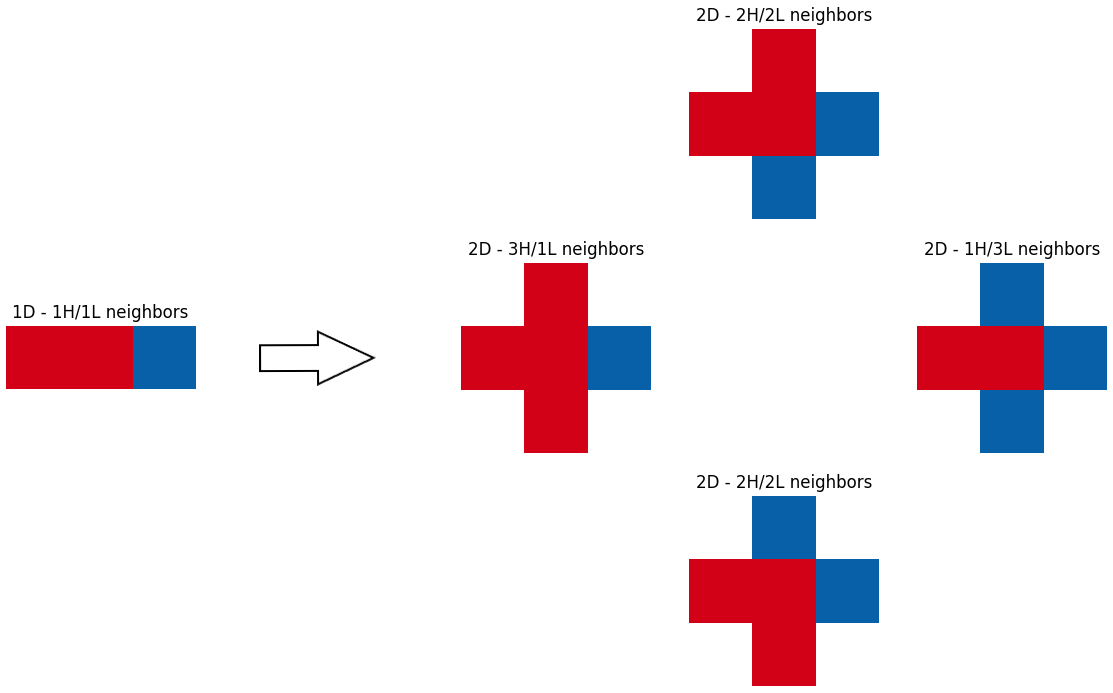
\includegraphics[width=0.85\textwidth]{figures/HHL_1D_to_2D.png}
        \caption{$HHL$ 1D sequence to 2D sequence}
        \label{fig:HHL_1D_to_2D}
    \end{subfigure}
    \hfill
    \begin{subfigure}[b]{1\textwidth}
        \centering
        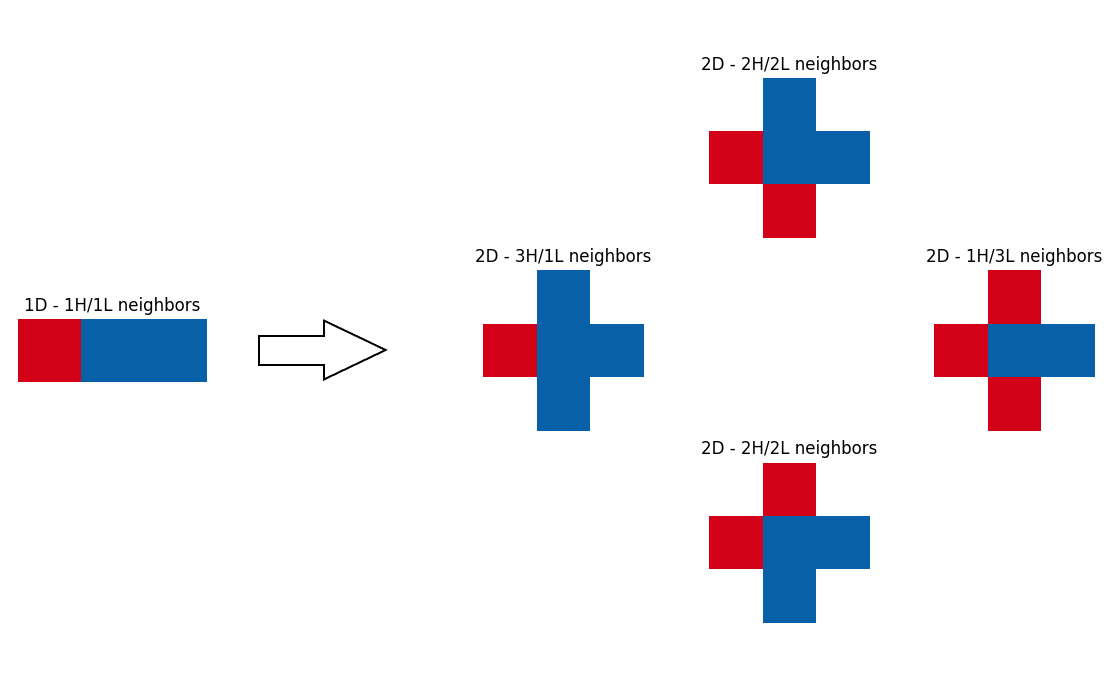
\includegraphics[width=0.88\textwidth]{figures/HLL_1D_to_2D.png}
        \caption{$HLL$ 1D sequence to 2D sequence}
        \label{fig:HLL_1D_to_2D}
    \end{subfigure}
    \caption{From initial 1D sequence to 2D sequence}
    \label{fig:1D_to_2D}
\end{figure}

\begin{itemize}
    \item First configuration when $u(x,0)=H$ (figure (\ref{fig:HHL_1D_to_2D})):
    
    In this configuration in 1D, the value at $t=1$ is different of the value at $t=0$,
    only if one of the neighbor is $H$ and the other is $L$. If both neighbors are $H$
    the value at $t=1$ is the same of the value at $t=0$. Taking in consideration the
    case when $u(x,0) \neq u(x,1)$, we want to know the similarity between the 1D and 2D
    sequences. In the figure (\ref{fig:HHL_1D_to_2D}) we can see that the 1D sequence
    can be represented as four 2D sequences whose two sequences has the same number of 
    neighbors $H$ and $L$. So we will defined the similarities between the 1D and 2D.
    Let's defined $N_H$ and $N_L$ as the number of neighbors $H$ and $L$ in the 2D sequence.
    Let's note the subtraction between $N_H$ and $N_L$ as $\Delta_{HL}=N_H-N_L$. 
    Then the formula is:

    \begin{equation}
        u_{2D}(x,y,t)=u_{1D}(\Delta_{HL} x,|\Delta_{HL}|t) 
        \label{eq:2D_1D_H}
    \end{equation}
    
    \item Second configuration when $u(x,0)=L$ (figure (\ref{fig:HLL_1D_to_2D})):
    
    The observations are the same as the first configuration, but we need to subtract 
    $N_L$ from $N_H$ to get the correct value. Let's note this subtraction as 
    $\Delta_{LH}=N_L-N_H$. Then the formula is:

    \begin{equation}
        u_{2D}(x,y,t)=u_{1D}(\Delta_{LH} x,|\Delta_{LH}|t) 
        \label{eq:2D_1D_L}
    \end{equation}
\end{itemize}

\subsubsection{2D formula using the 1D formula}

To summarize, we can find a formula to compute the value of concentration $u_{2D}(x,y,t)$
in the 2D sequence with the value of concentration $u_{1D}(x,t)$ in the 1D sequence. The
formula can be written as:

\begin{equation}
    u_{2D}(x,y,t)=u_{1D}(\Delta_N x,|\Delta_N|t) 
    \mbox{ where } \Delta_N=
    \begin{cases}
        \Delta_{HL}&\text{if }u_{1D}(x,0) = H\\
        \Delta_{LH}&\text{if }u_{1D}(x,0) = L\\
    \end{cases}
    \label{eq:2D_1D}
\end{equation}


\chapter{Future Work}

\section{Back-propagation of reflected wave}

When the propagation will reach the end of the sequence, a reflected wave will be
propagated back to the beginning of the sequence. As a consequence the two extrema get 
closer to each other to reach the stabilized state. If we take a sequence of $L$ with
$N$ elements, the end of the sequence is reached after $N$ steps. We know the value
of the wavefront when the end of the sequence is reached and just before the back 
propagation. We want to know the value of this wavefront when the back propagation
starts. Using the equations \eqref{eq:1D:normalized} and \eqref{eq:wavefront}
we can compute this value:

\begin{equation}
    \begin{split}
        u(N,N+1) & = u(N,N) + \alpha \left( u(N-1,N) - u(N,N) \right) \\
                 & = (1 - \alpha)u(N,N) + \alpha \times u(N-1,N)\\
                 & = (1 - \alpha)((1-\alpha^N)L+\alpha^NH) + \alpha \times u(N-1,N)
    \end{split}
    \label{eq:backprop}
\end{equation}
%
If $\alpha=1$ then $u(N,N+1)=\alpha \times u(N-1,N)$

\subsubsection{Assumption to verify}

We have the assumption that the back propagation at the end of the sequence is
like a flip of the start of the sequence. The concentration stays the same in the
sequence during the time (property \eqref{eq:associativity}). Before the back propagation
the start of the sequence is $u(-N,N)=H$ with $N$ the size of the $H$ sequence. At time
$N+1$ the back propagation starts and the concentration start to decrease 
($u(-N,N+1)<H$). While this concentration decrease the concentration at the end of the
sequence is increasing ($u(N,N+1)>L$). Our assumption is that the decreasing concentration
of the start of the sequence is the same as the increasing concentration of the end of the
sequence.


\section{Absorption of \texorpdfstring{$\mathrm{CO_2}$}{CO2} by the cells}

According to the article \cite{Aalto2002}, the $\mathrm{CO_2}$ flux in the leaf cells 
is influenced by several factors:

\begin{itemize}
    \item Light
    \item Temperature
    \item Ambient $\mathrm{CO_2}$ concentration
    \item Photosynthetic capacity of the mesophyll cells
    \item Size of the stoma opening
    \item Leaf structure
    \item Diffusion coefficients in the different parts
\end{itemize}

The $\mathrm{CO_2}$ concentration distribution is a continous sink and relatively constant 
over the airspace, but decrease rapidly in the mesophyll cells. Concentration inside the 
cells did not decrease more than 18\% from the value in the airspace. The article 
\cite{Kaldenhoff2012} says that the $\mathrm{CO_2}$ diffusion can be variable
in short time range, but it's a physical process dependant of structure so the 
diffusion rate is constant for time ranges of hours. This mecanism of $\mathrm{CO_2}$ 
diffusion is a matter of controversy vivid debate in the scientific community.

\subsubsection{Minimal model}

Consider a 1D sequence like on the section \ref{sec:stomata}. We will use the same sequence
of size 100 pixels but this time the end of the sequence will absorb $\mathrm{CO_2}$ and 
the rest of the sequence will diffuse it. We will assume that the diffusion is decrease by 
10\% in the mesophyll cells. In our sequence the ten last pixels will be the mesophyll 
cells. The formula for the diffusion does not change, but the diffusion rate is different. 
Indeed, the diffusion coefficient is different for the mesophyll cells pixels than for the 
rest of the sequence, it's equal to $0.9 \times \alpha$. With this rate of absorption by 
the mesophyll cells, we need $t=10236$ to obtain a concentration of 49\% instead of 
$t=8416$ without absorption. It takes 21\% more time to reach the stabilized state with 
10\% absorption than without absorption.

\subsubsection{Effect of absorption on stabilized concentration}

Because of the absorption phenomena the assumption \eqref{eq:associativity} is not true 
anymore. If the absorption is too high, the concentration will decrease too fast and the 
sequence will not reach the value of 49\%. For the sequence of 100 pixels, when the 
absorption is greater than 16\% the concentration at the end of the sequence will be less 
than 49\%. We want to plot the time taken to reach the value of 49\% at the end of the 
sequence for the different values of the absorption (see \textbf{Figure \ref{fig:absorb}}). We 
can see that the absorption influences a lot the time to reach a state near the stabilized 
state.

\begin{figure}[h]
    \center
    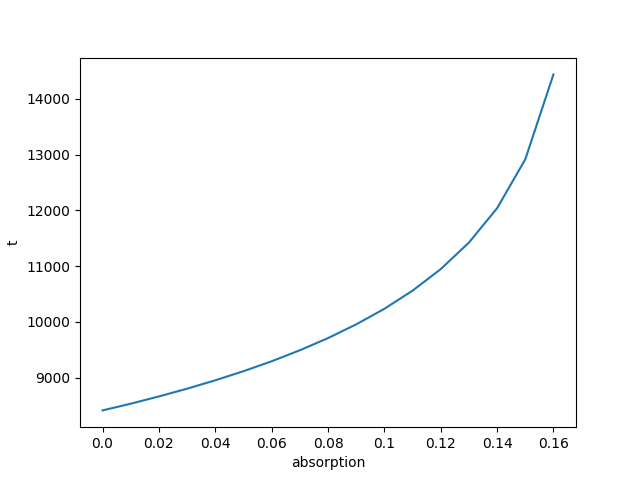
\includegraphics[width=0.66\textwidth]{figures/absorption.png}
    \caption{Time to reach the value of 49\% at the end of the sequence for different values of absorption}
    \label{fig:absorb}
\end{figure}

\chapter{Conclusion}

To conclude, this internship was a great opportunity to learn about the research process 
and to get a taste of what it is like to work in a research group. I have learned a lot 
about the research process and about the different tools that are used in. I have also 
learned a lot about research that are done in the field of computer vision, pattern 
recognition, and some other areas that are interesting to me. During this internship,
I wrote my first scientific paper for a workshop organized by the Austrian Association 
for Pattern Recognition (OAGM) \cite{OAGM}. Currently, I don't know yet if the paper
is accepted or not, but I prepared a poster for the workshop if the paper is accepted.
It was a very good experience to write a paper and a poster, and I hope I could
participate to the workshop if the paper is accepted.

\cleardoublepage
%\pagebreak
\phantomsection
\addcontentsline{toc}{chapter}{Acknowledgements}
\chapter*{Acknowledgment}
\vspace{1.0in}

I'm extremely grateful to Walter G. Kropatsch for giving me the opportunity to make this
internship in the PRIP laboratory. I would also like to thank him for his passion for 
research and the way he has transmitted it. I'd like to express my deepest thanks to
Jiří Hladůvka who was my supervisor during the internship. He gave me a lot of good
advice and helped me to understand the research process. I would also like to thank
Majid Banaeyan and Darshan Batavia for their help and support during the internship.
I would like to pay my special regards to Samuel Peltier for giving me the contact
of the PRIP laboratory. I must also thank Thierry Urruty my supervisor in France.
Finally, I would like to thank all the people I have met during the internship and
the friends I have made in Vienna.

\newpage

\cleardoublepage
%\pagebreak
\phantomsection
\addcontentsline{toc}{chapter}{References}

\bibliographystyle{habbrv}
\bibliography{refs}

\listoffigures

\listoftables


\end{document}
